
\chapter{BACKGROUND}

\graphicspath{ {./background/} }
%%%%%%%% This line gets rid of page number on first page of text
\thispagestyle{empty}

%%%%%%%%%%%%%

\section{The Rise of Machine Learning}

%Artificial Intelligence (AI) is democratized in our everyday life%
Machine learning now affects many aspects of our lives from web searches, streaming services, recommendations on e-commerce websites, smart speakers, stock predictions to criminal justice and healthcare systems. It is omnipotent in consumer products such as cameras, smartphones and personal assistants. There is a huge incentive for businesses to apply machine learning from enhanced decision making, business forecast, cost reduction, risk management, productivity improvements, as well as the development of new products and services.

Machine learning is a branch of computer science that uses statistical techniques to give computer systems the ability to learn from data, find patterns in data and make highly accurate predictions. In other words, its a set of techniques used to teach computers how to learn, reason, perceive, distinguish, infer, communicate and make decisions like human do. It is a large part of modern artificial intelligence (AI). Here, data encompasses many things such as words, numbers, images, video and more. Machine learning learns from the experience, following a pathway that nature took millions of year ago \cite{sejnowski2018deep}. It's a paradigm shift from programming where all the instructions must be given explicitly to the computer, to 'indirect' programming where the computer learns patterns from the data without being explicitly programmed.

Not very long ago, to say that computer vision could compete with the visual abilities of a one-year-old was unrealistic. It is no longer the case \cite{sejnowski2018deep}. Machine learning techniques can now recognize objects in an image as well as an adult can, digitize handwritten characters, transcribe speech into text, classify wine types, support diagnosis of severe diseases, match news item or product with user's interest and select results relevant to the search. Then there are self-driving cars on the road that can drive more safely than an average person \cite{sejnowski2018deep}.

What is fuelling these advances is the recent surge in data, the rise in computing power over the past few years and faster algorithms, which has led to breakthroughs in the field of machine learning. These three are the essential ingredients that lead to the emergence of deep learning revolution \cite{gerrish_how_2018}.

\begin{figure}[htbp]
\centering
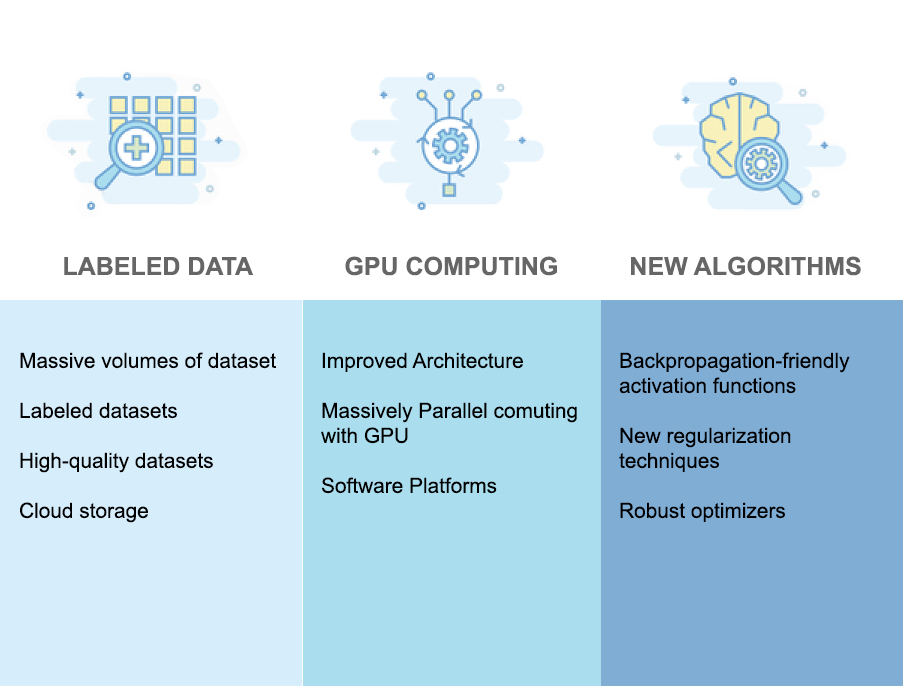
\includegraphics[width=0.90\textwidth]{images/bg-drive-factors.png}
\caption{Three factors powering current advancement in machine learning}
\label{3-factors}
\end{figure}

\subsection{Data Upsurge}
The exponential growth in data in recent times has fueled machine learning based industries, technologies, and services. Nonetheless, humans and machines are generating more data today than ever before. Every day, humans alone produce a massive amount of data ranging from text, audio, video, sensory data and more, and that number is expected to proliferate in the decades to come. 

Another example of this is a modern car that has more than 100 sensors to monitor multiple functions such as fuel level, radar sensors and ultra sensors for close range detections.

\subsection{Computing Power}
Thanks to Moore’s law, processor chips continue to shrink in size, while increasing computing power, which has risen three to four magnitude compared to mid-1990s. The advance in computational power that has inevitably made all this possible derives not only from Moore’s law but also from the discovery of graphics processing units (GPU)s. 

GPUs were first designed to boost speed and processing power in gaming industries give gamers a rich, high-speed 3D visual experiences \cite{Yosinski2015}. These were found to be twenty to fifty times more efficient than traditional central processing units (CPUs) for machine learning and deep learning computations.

Open AI, a non-profit research organization that promotes AI safety, remarks\cite{aicompute} - \begin{quote}
    \textit{Improvements in computing have been a key component of AI progress, so as long as this trend continues, it’s worth preparing for the implications of systems far outside today’s capabilities.}
\end{quote}

An example of this is in speech recognition, where a computer has to perform millions of calculation per second for a system to learn and recognize patterns in the data — This task required tremendous computational power that, until quite recently wasn't available. In contrast, Marvin Minsky, a pioneering mathematician, leading scientist and the founder of MIT Artificial Intelligence Laboratory (MIT AI Lab) worked on AI in 1957 when computers were billions of time slower than they are now \cite{ubiquitous_ai}. Those machines were costly and provided merely a fraction of the performance and computing speed.

\subsection{Inventive Algorithms}
%TODO: Consider Changing to - Algorithmic Innovation%
The data explosion and advances in computing power has made it possible for better and refined algorithms, and enable more extensive datasets that algorithms can process at any given time for machine learning tasks. 

Traditionally, algorithms were programmed explicitly by humans to perform various tasks. Modern algorithms have become sophisticated to the point where they can facilitate machine learning and allow computers to self-learn from the data. Until recently there hasn't been adequate data, either structured or unstructured to train computers to perform complex tasks on their own, let alone develop sophisticated algorithms that allowed machines to train themselves. 

An example of this is the autonomous vehicles car that rely on an enriched visual dataset to construct their own map real-time and navigate the roads \cite{shannon_mattern} \cite{tesla_autopilot}. Here, each frame of the video collected by a self-driving car must be enriched with data to identify objects such as a road sign, pedestrian, tree or sidewalks, in every frame.

According to AI expert and MIT Sloan professor Erik Brynjolfsson \cite{hbr_ai_business}, there has been some significant improvements of these algorithms in the field of machine learning that have improved on the basic algorithms. Some of them were first introduced 30 or 40 years ago, but they have now been tweaked and improved by the virtue of faster computing and huge volumes of data. This makes it more convenient to figure out what works and doesn't work over time.

These three things combined, computing power, volumes of data and better algorithms could provide as much as a million-fold improvement on some application from image recognition and speech synthesis to self-driving cars.

\section{The Dawn of Neural Networks}
In mid-1990, Artificial neural networks were introduced by researchers \cite{efron2016computer}, and they marked a paradigm shift of predictive modeling from the world of applied statistics towards computer science and machine learning.

\section{Deep Learning Revolution}

Deep learning is a super set of the machine learning that has its root in mathematics, computer science and neuro-science. Above all, mathematics has an essential role in deep learning as it is in the study of visual processing of brain. Neural networks were reincarnated around 2010 with “deep learning” as a new name, largely a result of much faster and larger computing systems, in addition to some new ideas. \cite{efron2016computer}.

\iffalse
\begin{figure}[htbp]
\centering
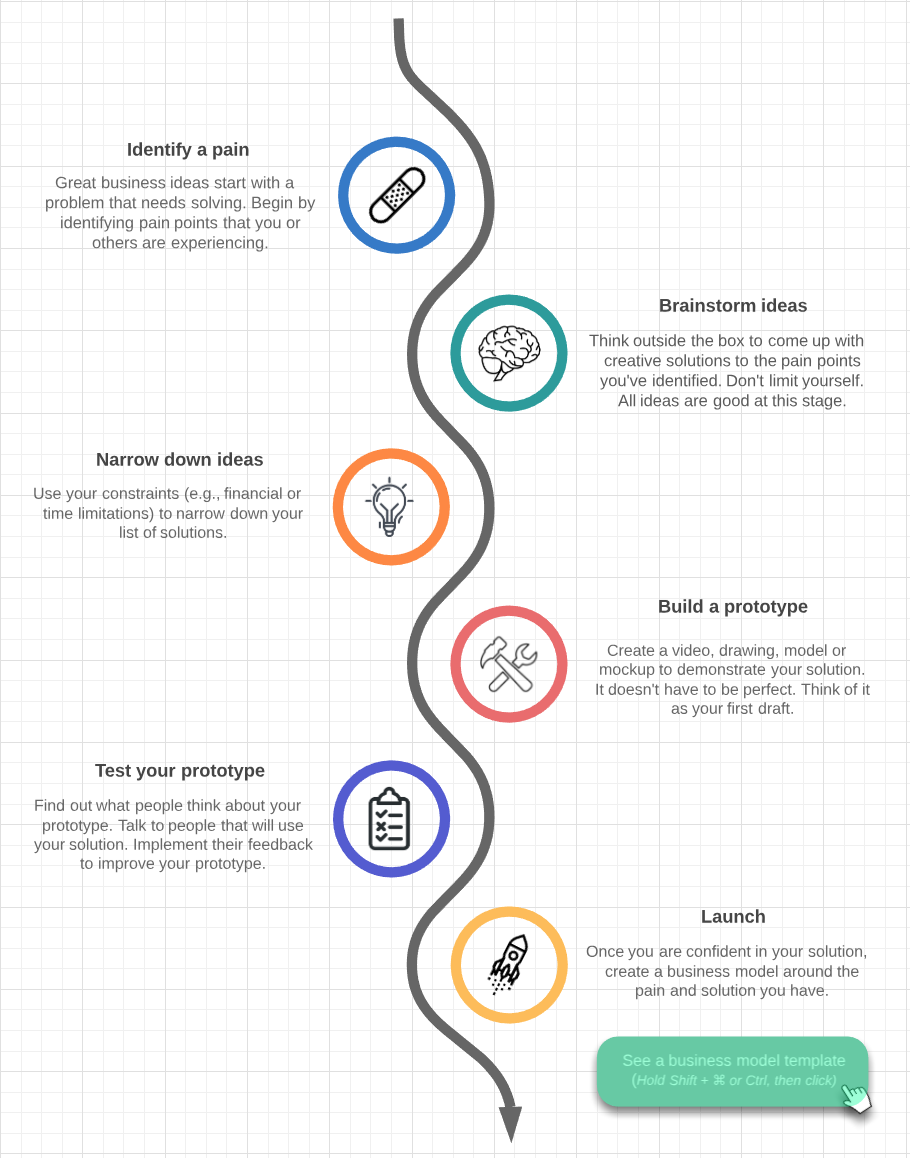
\includegraphics[width=0.85\textwidth]{images/timeline-1.png}
\caption{History and Timeline}
\label{fig:timeline}
\end{figure}
\fi

Deep learning \cite{Polson2018} is a specific set of techniques from the broader field of machine learning that focus on the study and usage of deep artificial neural networks to learn structured representations of data. It is used for classifying patterns using large training data sets and multi-layer neural networks. It's primarily a method for machines to learn from data that are loosely modeled on the way a biological brain learns to solve problems \cite{pavlus_john}, where each artificial neural unit is connected to many other such units, and the links can be statistically strengthened or decreased based on the data used to train the system. Each successive layer in a multi-layer network uses the output from the previous layer as input.

The origin of deep learning goes back to the birth of artificial intelligence in the 1950s, when there were two competing visions for how to create an AI: one vision was focused on symbolic approaches based on logic and computer programs, which dominated AI for decades; the other was based on learning directly from data, which took much longer to develop and show results \cite{sejnowski2018deep}.

In 1956, John McCarthy, a Mathematics Professor at Dartmouth College proposed a workshop called Dartmouth Summer Research Project on Artificial Intelligence \cite{edselc.2-52.0-3384609253620061201}, which gave birth to the field of AI and motivated a generation of scientists and experts to explore the untapped potentials for information technology to match the capabilities of humans \cite{sejnowski2018deep}.

In 1956, Psychologist Frank Rosenblatt at Cornell University, aimed to create brain analogue useful for analytical tasks \cite{2016397}.  He invented a simple technique for simulating neuron in hardware and software. This marked the inception of the research in field of enabling machines to learn and classify in human. Rosenblatt proposed ‘perceptron’ a single layer neural network for binary classification that could learn how to sort simple images into categories - for instance, squares and triangles. Perceptron went on to be the basis of further research that culminated into the creation of multi-layer learning networks, which have formed the basis of modern deep learning\cite{2016397}.

In the last decade, deep learning has been successfully applied to a variety of domains and applications \cite{dl_evolution} that require large volumes of digital data for training and providing useful information. Recently, they have has been advancing the state-of-the-art in artificial intelligence, and had led to major breakthrough in many areas such as computer vision (CV) \cite{krizhevsky2012imagenet} \cite{karpathy2014large}, speech recognition \cite{graves2013speech} \cite{mohamed2012acoustic}, and natural language processing \cite{bengio2003neural} \cite{mikolov2013distributed} \cite{mikolov2010recurrent}.

\section{Architecture Overview}

Now that we have seen various components of deep neural networks, this section gives a broader overview of the four major architectures of deep networks.

I broadly survey the types of neural network to provide general insight and take a look some of the major vision based architecture of deep neural networks with application in industry and academia. 

\begin{itemize}
\item Perceptron
\item  Multi-layered Perceptron
\item Convolutional Neural Networks (CNN)
\end{itemize}


\subsection{Perceptrons}

A neural network is a highly parametrized model \cite{efron2016computer}, inspired by the architecture of the human brain. It was widely promoted as a universal approximator—a machine that with enough data could learn any smooth predictive relationship.

\subsubsection*{Single Layer Perceptrons}

A single-layer perceptron or feed-forward neural network is a collection of neurons arranged in a sequence of multiple layers, where each neuron receive as input from the previous layer and perform a simple calculation (e.g., compute a weighted sum of the input followed by a nonlinear activation function) \cite{efron2016computer}. The neurons of the network collectively perform a nonlinear mapping from the input data to the output data. This mapping feature is learned from the data by adjusting and adapting the weights of each neuron using a technique called backpropagation \cite{efron2016computer}.

Perceptron structure is illustrated in Fig.~\ref{fig:perceptron}.

\begin{figure}[htbp]
\centering
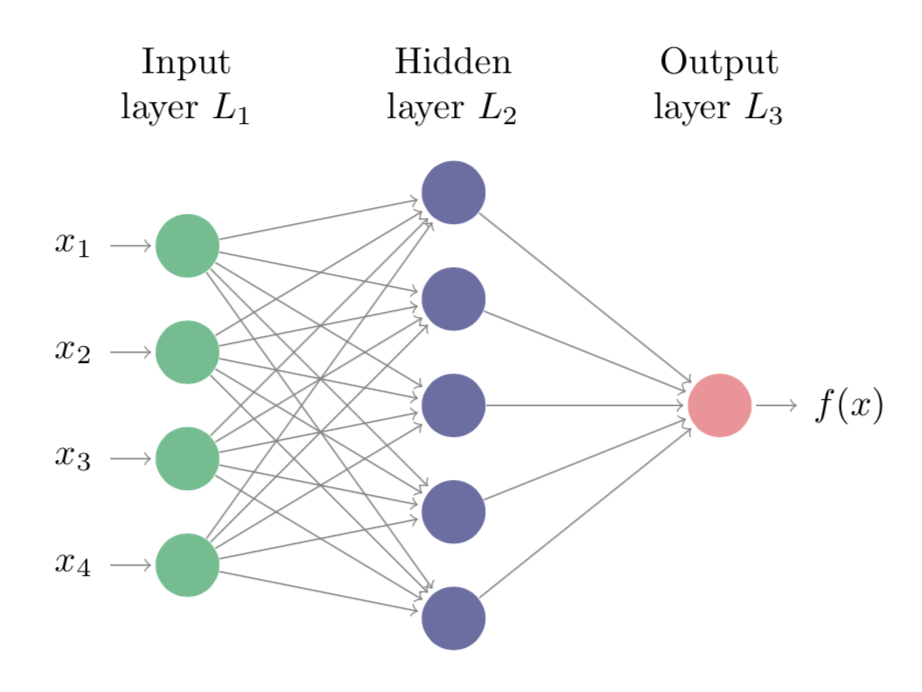
\includegraphics[width=0.6\textwidth]{images/perceptron.png}
\caption{Neural network diagram with a single hidden layer. The hidden layer derives transformations of the inputs—nonlinear transformations of linear combinations—which are then used to model the output.}
\label{fig:perceptron}
\end{figure}

\subsubsection*{Multi Layer Perceptrons}

Figure 2.2 shows a simple example of a feed-forward neural network diagram. There are four predictors or inputs, five hidden units and a single output unit:

\begin{equation}
a_{l} =g\left( w^{( 1)}_{l0} +\sum\nolimits ^{4}_{j=1} w^{( 1)}_{lj} x^{j}\right)
\label{four input units and five hidden units}
\end{equation}

The hidden layer derives transformations of the
inputs—nonlinear transformations of linear combinations—which are then used to model the output, and there is a single output unit:

\begin{equation}
 o=h\left( w^{( 2)}_{0} +\sum\nolimits ^{5}_{l=1} w^{( 2)}_{l} a_{l}\right)
 \label{single output units}
\end{equation}

Feed Forward Neural Network Fig.~\ref{fig:multi-layer}.
\begin{figure}[htbp]
\centering
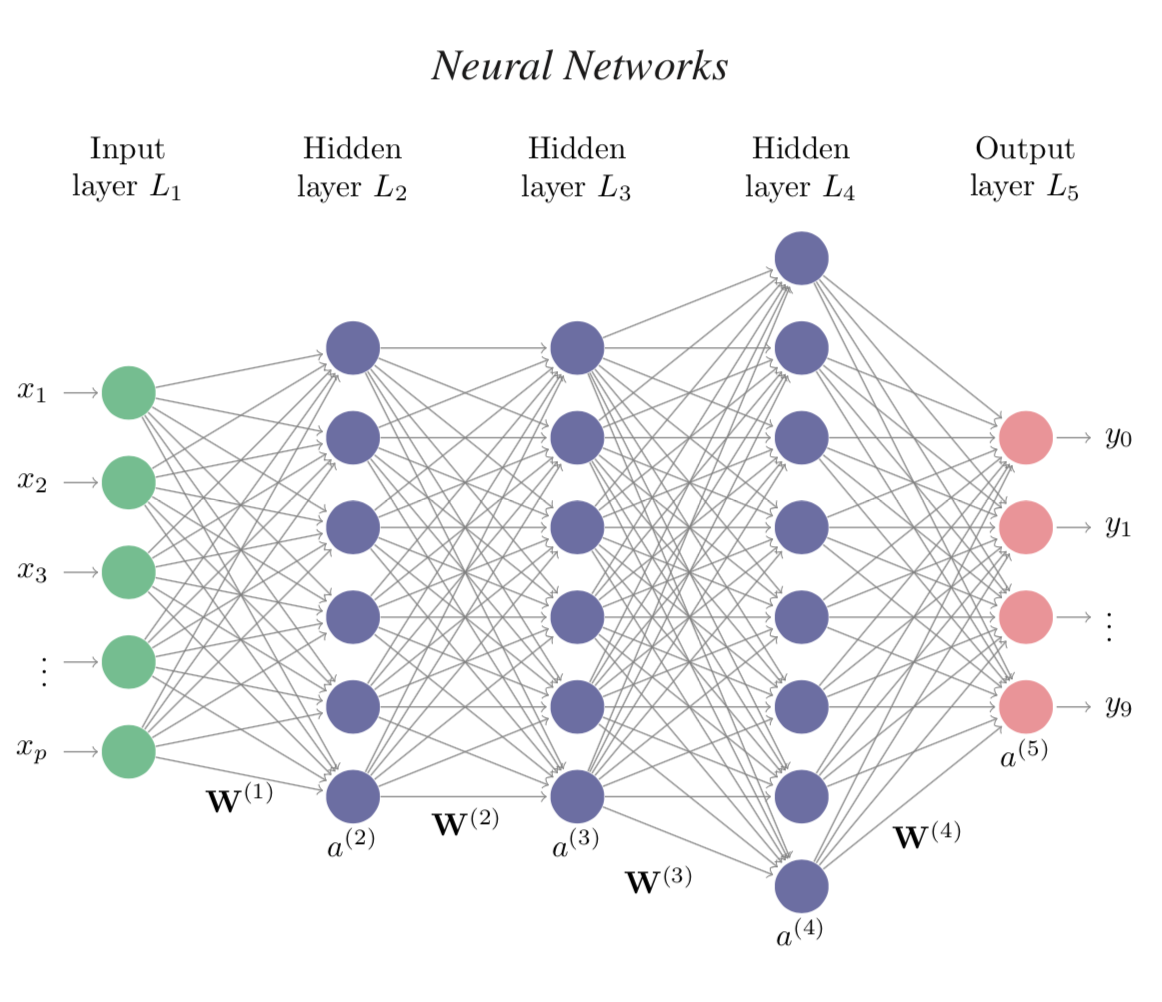
\includegraphics[width=0.75\textwidth]{images/NN.png}
\caption{Neural network diagram with three hidden layers and multiple outputs, suitable for the MNIST handwritten-digit problem. The input layer has p D 784 units. Such a network with hidden layer sizes .1024; 1024; 2048/, and particular choices of tuning parameters, achieves the state-of-the art error rate of 0:93.}
\label{fig:multi-layer}
\end{figure}

\clearpage

\subsection{Convolutional Neural Networks}
A convolutional neural network (CNN) is a feed-forward artificial neural network in which the network preserves the hierarchical structure by learning internal feature representations and generalizing the features in the common image problems such as image classification tasks. It is not restricted to images; it also applied in natural language processing problems and speech recognition \cite{Manaswi2018}.

\begin{figure}[htbp]
\centering
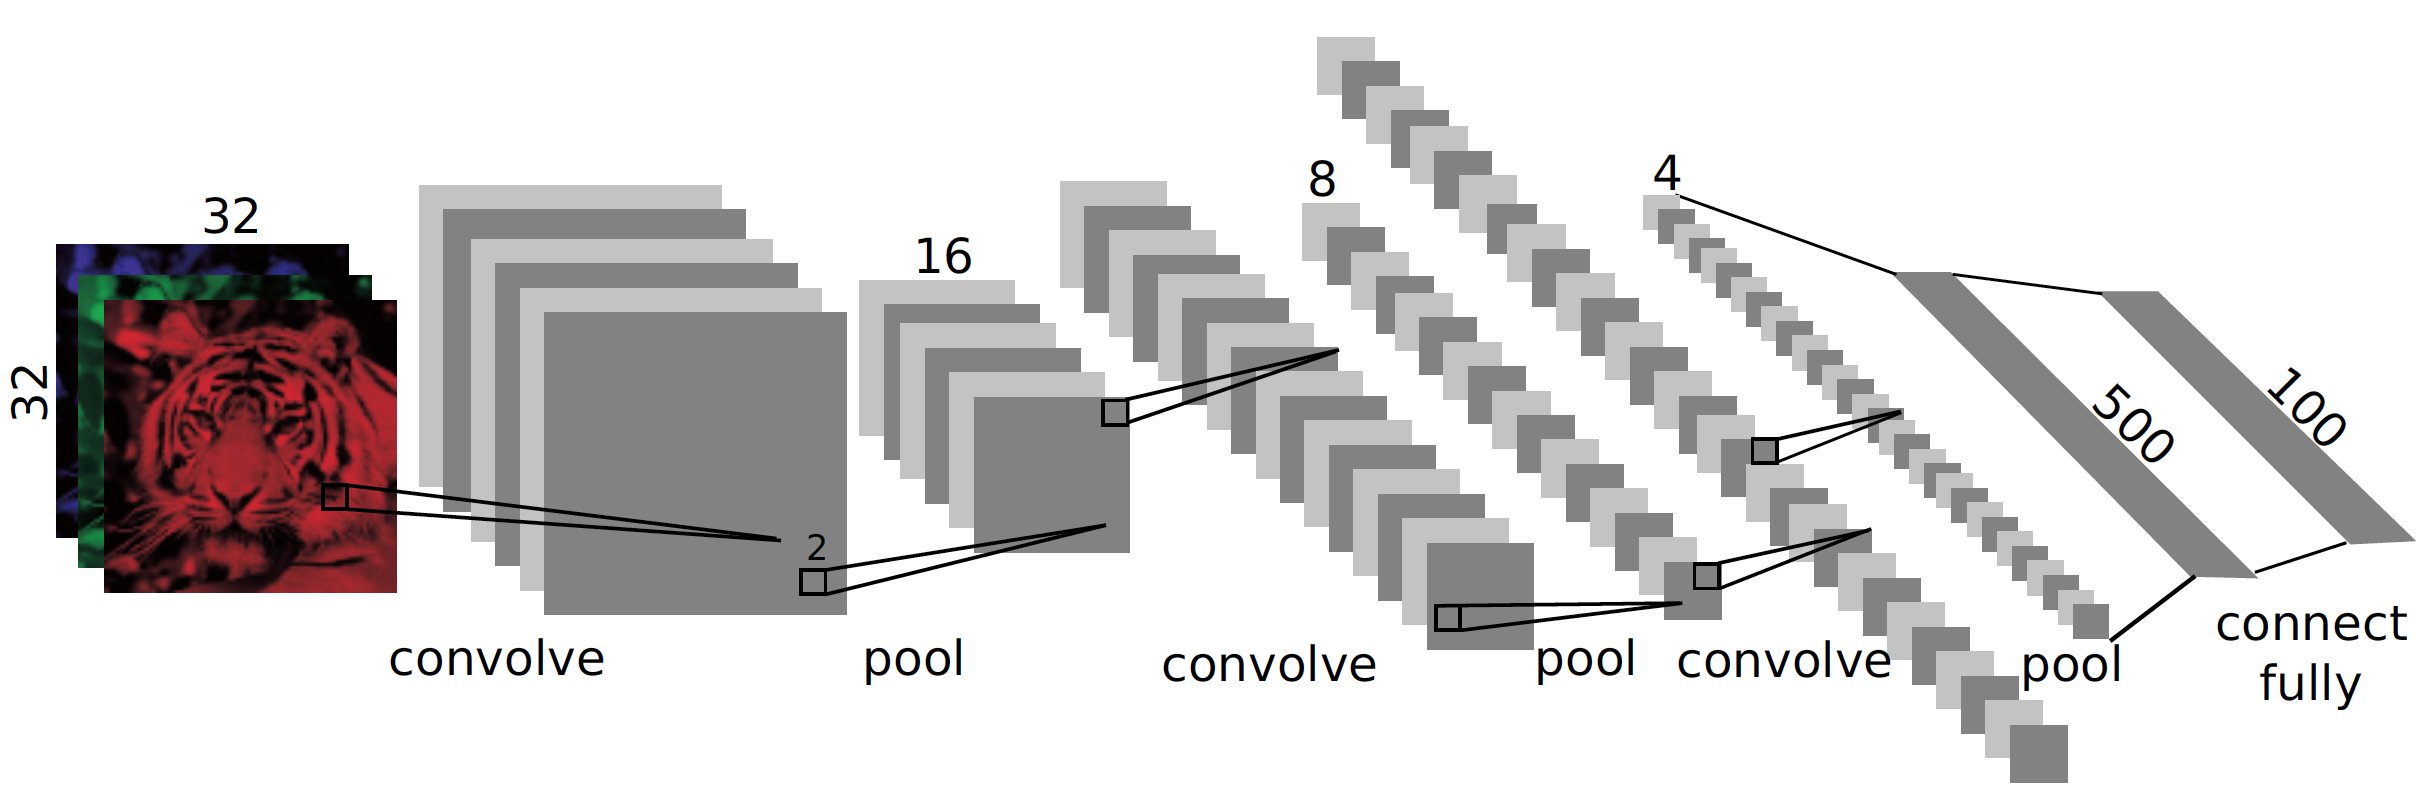
\includegraphics[width=0.90\textwidth]{images/cnn-arch-1.png}
\caption{Network architecture and different layers}
\label{fig:CNN-1}
\end{figure}

A classic network architecture of CNN is comprised of stacked convolutional layers, periodically followed by a pooling layer, activation function, and optional batch normalization. It also consist of the fully connected layers. As an image moves through the network, it's spatial dimensions are periodically down-sampled while increasing the number of feature maps. The final layer outputs the class probabilities prediction.

These architectures can be broadly classified as classic network architectures such as, LeNet-5, AlexNet and VGG16, and modern network architectures such as Inception, ResNet, ResNeXt and DenseNet. While the classic network architectures are mainly comprised of stacked convolutional layers and few fully connected layers, the latest state-of-the-art architectures explore innovative techniques for constructing convolutional layers that allows for more efficient learning.

These architectures serve as baseline to build on top of them to solve various computer vision tasks. These architectures serve as rich feature extractors which can be used for computer vision problems such as object detection \cite{edseee.690947520140101}, object tracking, pose estimation, text detection, visual saliency detection, semantic segmentation \cite{edseee.690947520140101}, image captioning \cite{edsarx.1411.455520140101} \cite{edsarx.1411.495220140101} \cite{edseee.778086320160101}, visual question answering \cite{edseee.741063620150101} \cite{edsarx.1505.0561220150101} \cite{Wongsuphasawat2018}, action recognition, scene labeling, speech and natural language processing. 

The effectiveness of CNN in image recognition is one of the main reasons why the world recognizes the power of deep learning. As Figure 4-7 illustrates, CNN is good at building a position and rotation invariant features from raw image data. It has lead to significant advances in machine vision, which has critical applications for self-driving cars, robotics, drones, and treatments for the visually impaired.

A simple example of a computer vision model Fig.~\ref{fig:CNN-2}.
\begin{figure}[htbp]
\centering
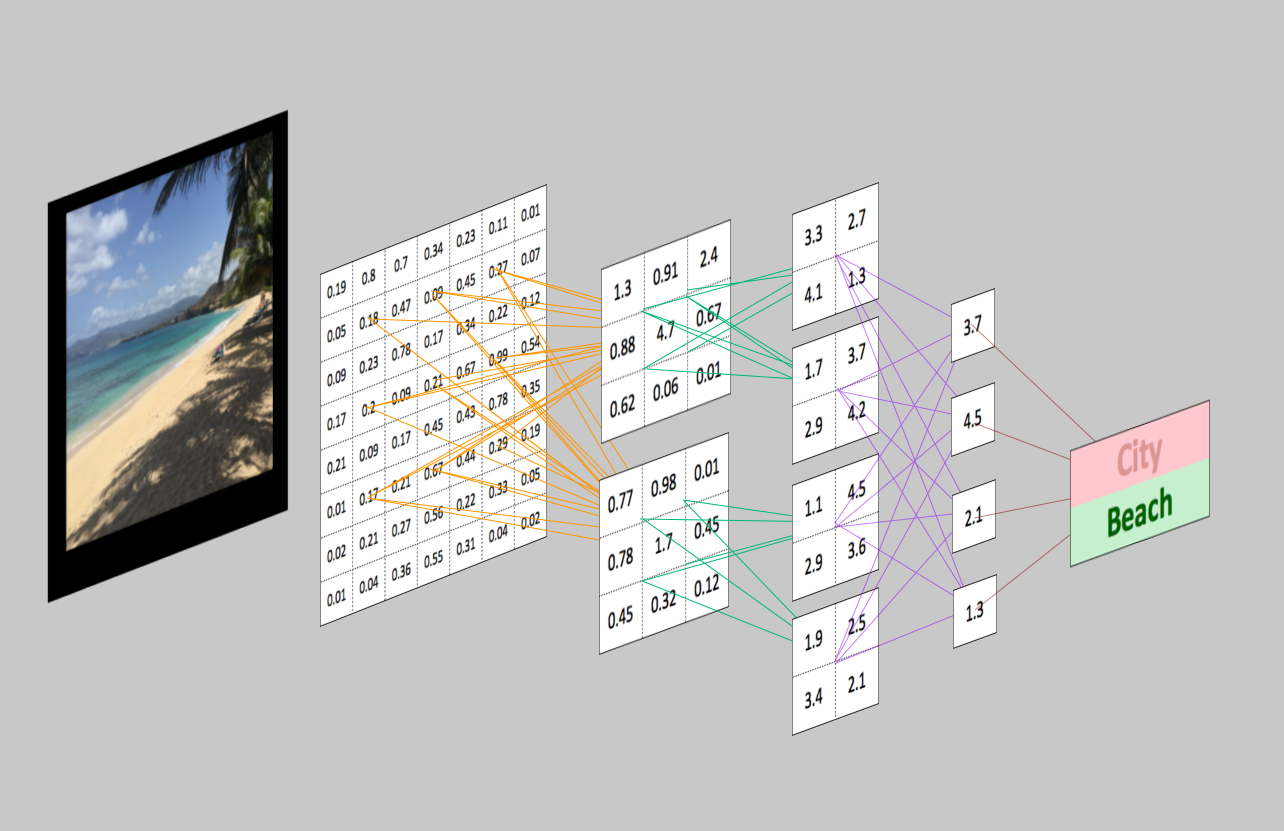
\includegraphics[width=0.75\textwidth]{images/CNN.png}
\caption{Computer Vision Example}
\label{fig:CNN-2}
\end{figure}

The broad range of CNN model families include (1) CNNs with fully-connected layers (e.g. VGG), (2) CNNs used for structured outputs (e.g. captioning), (3) CNNs used in tasks with multi-modal inputs (e.g. VQA) or reinforcement learning.

\vspace{15mm}

\subsection{Tasks}
\begin{itemize}
\item Classification
\item Regression
\item Similarity Matching
\item Clustering
\item Co-occurrence grouping
\item Profiling
\item Link prediction
\item Data Reduction
\item Causal Modelling
\end{itemize}

\subsection{Types of Learning}

There are different types of learning process. Learning can be supervised, semi-supervised, unsupervised and reinforcement.

\subsection*{Supervised learning}

Supervised learning \cite{sammut2011encyclopedia} refers to training a model using a labeled dataset, where some of the training examples have labels, but others don’t. It's a machine learning process that learns a function from an input type to an output type using data comprising examples that have both input and output values. Two typical examples of supervised learning are classification learning and regression. In these cases, the output types are respectively categorical (the classes) and numeric. 

\subsection*{Unsupervised Learning}

Unsupervised learning \cite{sammut2011encyclopedia} refers to any machine learning process that seeks to learn to find patterns in a dataset, typically an unlabeled dataset or learn structure in the absence of either an identified output. The typical examples of unsupervised learning are clustering, dimensionality reduction, recommendation and self-organizing maps.

\subsection*{Reinforcement Learning}

Reinforcement learning \cite{sammut2011encyclopedia} refers to a large class of learning problems characteristic of autonomous agents interacting in an environment: sequential decision-making problems with delayed reward or involving reward maximization. Reinforcement-learning algorithms seek to learn a policy (mapping from states to actions) that maximizes the reward received over time.

Unlike in supervised learning problems, in reinforcement-learning problems, there are no labeled examples of correct and incorrect behavior. However, unlike unsupervised learning problems, a reward signal can be perceived. This technique is based on the way animals seem to learn in response to positive feedback and requires a massive amount of dataset \cite{sammut2011encyclopedia}.

\section{The Advent of Black Box Models}

Deep learning models are harder to interpret than most existing machine learning models \cite{Kahng2018} because of its large number of layers and parameters, multiple types of non-linear activation functions and randomized gradient descent training process, understanding these models remains a fundamental challenge and because of this, the deep neural network is often considered as “black box \cite{dlvwz}.” Although there has been some effort lately in the machine learning and human-computer interaction community to shed light on their inner-workings, most observers would acknowledge that neural networks as a whole remains a black box.

\begin{figure}[htbp]
\centering
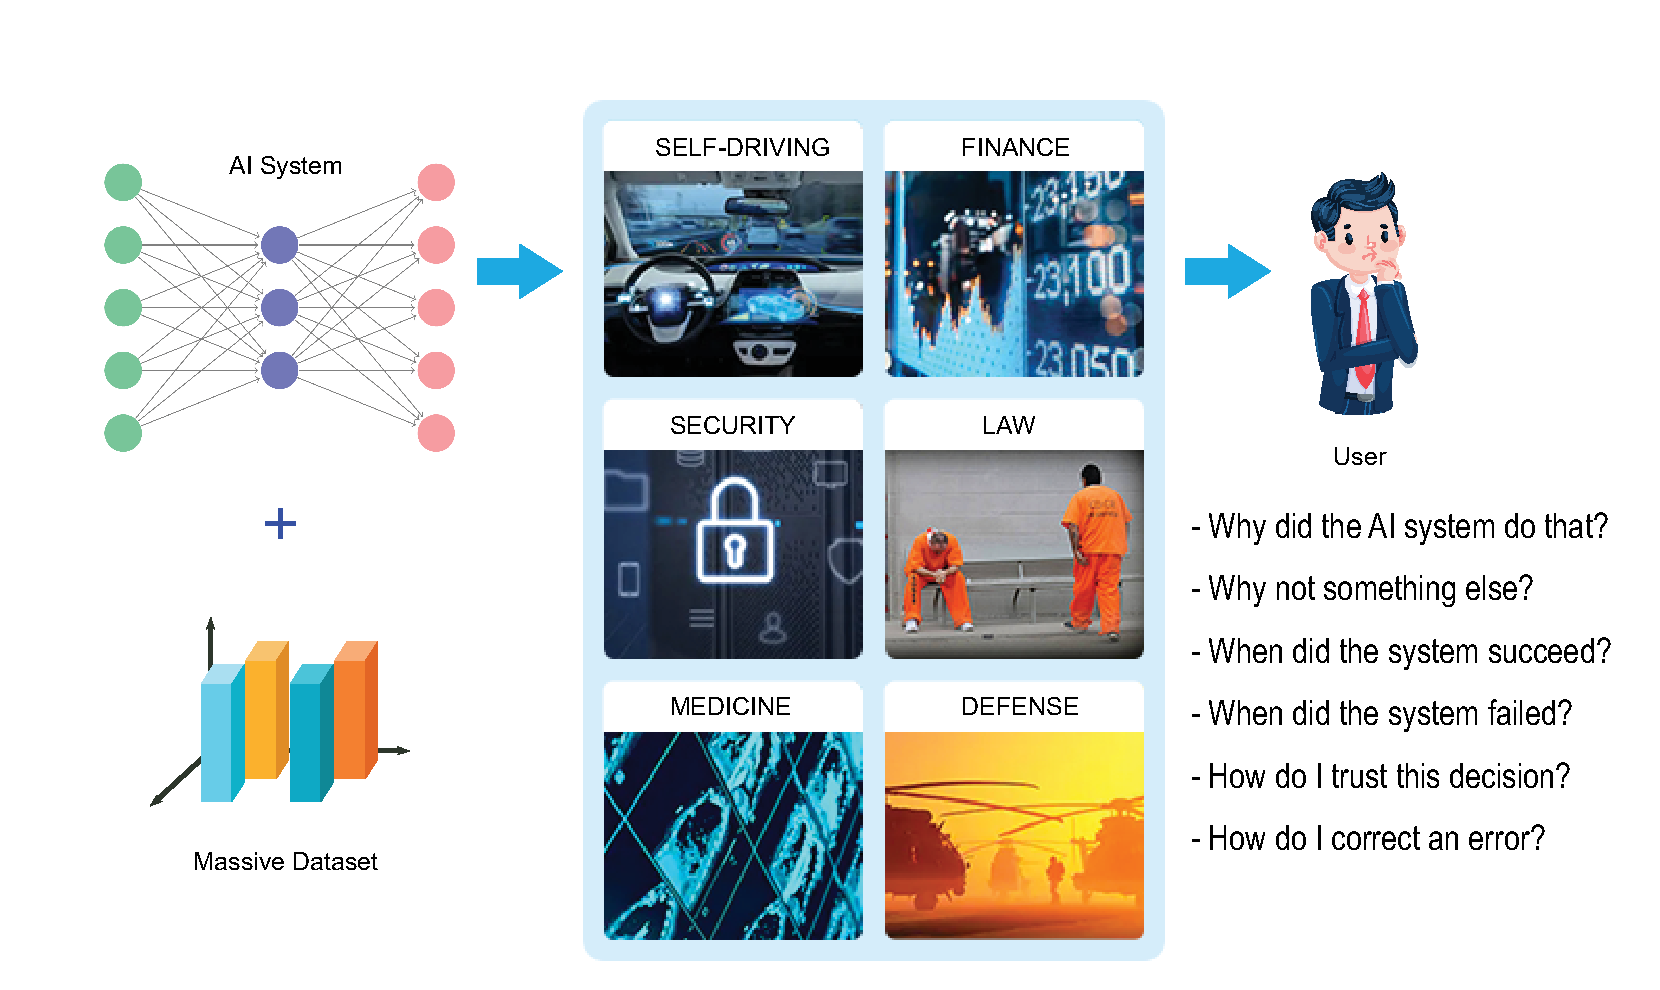
\includegraphics[width=1\textwidth]{images/Blackbox-AI-copy.eps}
\caption{Blackbox AI System}
\label{fig:Blackbox AI system}
\end{figure}

Due to their internal complexities and non-linear structure \cite{Samek}, the underlying decision-making processes for why the models are achieving such performance are the challenge and sometimes mystifying to interpret. Therefore, in practice, users often approach them as a black box and cannot explain how learning from input data was done nor how performance can be consistently optimized due to which the development of the model largely depends on the trial-and-error process. It could also be detrimental when the model does not perform satisfactorily; users are not able to understand the causes or know how to fix the problem. 

Generally, the information stored in a neural network is a set of numerical weights and connections that provide no direct evidence as for how to the task is executed or what is the association between inputs and outputs \cite{Tzeng2005}. The opaque nature of these models also limits their usage and acceptance in high-end science and engineering applications since it is demanded to use methods and techniques based on functions that can be understood and validated.

Another reason that complicates the use of the neural network is that there are no well-defined criteria for choosing a neural network structure and corresponding parameter selection \cite{dlvwz}. It mostly depends on the trial and error process. The appropriate selection of parameters can vary widely even when performing very similar tasks due to various reasons. These parameters, which include network structure, depth and width of hidden layers, error bound, learning rate, training algorithm, hidden layer size, and the data vector used are often selected in a trial-and-error process. Therefore, when designing neural networks, it is tough for beginners to select the right parameters and find correct general rules. While, even for deep learning experts, it largely remains a trial-and-error process.

\begin{figure}[htbp]
\centering
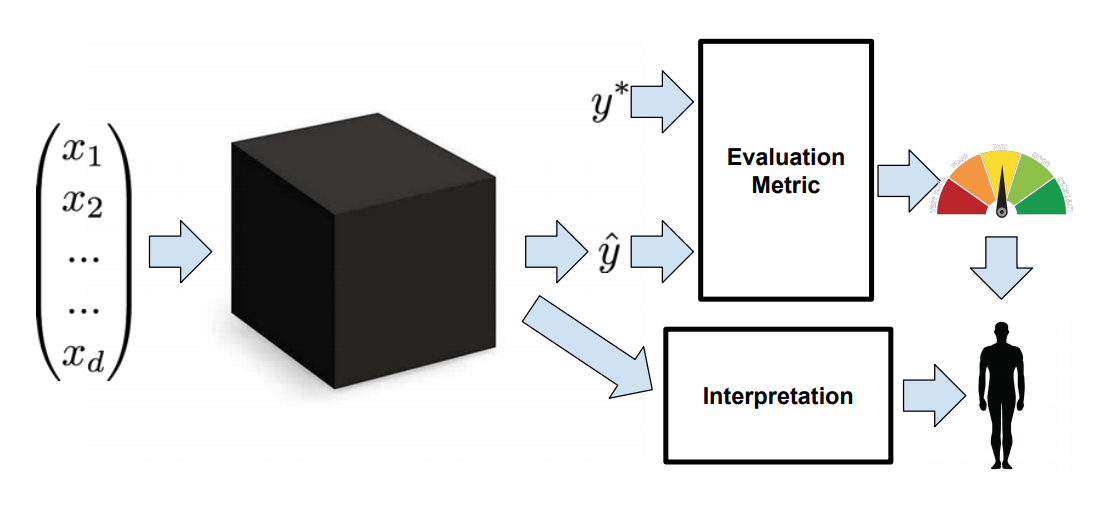
\includegraphics[width=0.90\textwidth]{images/Black-box.png}
\caption{Black box example of neural network system}
\label{fig:blackbox}
\end{figure}

The problem stems from the fact that we cannot merely inspect the deep neural network to see how it works or how it performs parallel computations \cite{darksecretaimittr}. A network’s learning and reasoning are embedded in the behavior of thousands of simulated neurons, arranged in dozens or even hundreds of intricately interconnected layers. 

For example, in the CNN model, neurons in the first layer receive an input image (as RGB value), which performs computation and outputs a new signal. These signals are fed into the successive layer and so on until the final layer output is generated \cite{darksecretaimittr}. Additionally, there is a process known as backpropagation that adjusts the calculation of neurons to optimize the output. The backpropagation algorithm is the standard training method which uses gradient descent optimization to update the parameters.

Further, traditional analysis with dense network is complicated because of the intricate array of high dimensional data involved. Advanced algorithms discern so many varied patterns in the dataset, which they leverage to make decisions. The user has an idea about what went in but has no idea about what patterns were recognized or were most significant to arrive at the solution that was given out.

\section{Societal Implications}

AI has been democratized in our life, and now permeates every aspect of our social lives from the social media platforms, streaming services, smart-speakers to healthcare system. It is now deeply embedded in various business decisions, both routine and high stakes because they promise to provide superior performance and improve the consistency and quality of the decision-making. 

These techniques have also been embraced in regulated domains such as employment, credit, and insurance, where critical decisions like who gains access to healthcare, who’s approved for a loan, who gains access to critical opportunities and criminal risk assessment \cite{ainow2018} depends on the output of the machine learning model. Yet there is a perception and emerging concern that these learning algorithms from historical data can end up encoding human biases and prejudice they promised to alleviate.

Over the past few years, algorithmic bias and fairness question has become a matter of concern for consumer advocates, regulators, policymakers, civil right groups and even businesses. Society is built upon a fabric of expected behavior and mutual trust \cite{Lipton2018}. In order for these models to be accepted by society, they need to know the rationales for their decision and understand know why they’re making the decisions they’re making. It is also important we design AI systems that respect and fit with the social norms and ensure that their decision making is consistent with the ethical judgment and human rights.

With the growing influence of AI and their prevailing impact on the public domain, there is a critical need to better understand their decisions and realize how these models operate.  In a societal context, the reasons for a decision matters a lot. For example, death caused intentionally (murder) vs. death caused unintentionally (manslaughter) are distinct crimes at the court of law. Similarly, a hiring decision made is based (directly or indirectly) on specific protected characteristics such as race, the socio-economic class has a bearing on its legality. However, currently, predictive models are not capable of reasoning this or provide any kind of explanation to their decisions \cite{molnar}.

In this section, I examine the social implications of the black box model, including how the relative opacity of the model is potentially endangering the social equality and its wide-ranging impact on various social domains. I focus my discussion on the societal implication through six critical themes:

\begin{enumerate}
\item \textbf{Trust}
\item  \textbf{Transparency}
\item \textbf{Fairness and Inclusion}
\item \textbf{Ethics}
\item \textbf{Privacy}
\item \textbf{Safety}
\end{enumerate}

We selected these themes because they are overarching concerns in the public domain. We discuss the harmful effect in each of these areas and identify emerging challenges in the present and future. In our discussion about these themes, we also ask the underlying questions such as: what are the current social and economic challenges faced by the rapid integration of AI, and how we can build a deeper understanding of AI \cite{Solon2017} in the present time that will help us create a fair and equitable future?

\begin{figure}[htbp]
\centering

\includegraphics[width=1\textwidth]{images/societal-impact-copy.eps}
\caption{Societal implications of the black box system}
\label{fig:societal-impacts}
\end{figure}

The wide-ranging impact in these selected themes makes it essential to look at how these automated decision-making systems are being applied now in regulated industries, whom they are benefiting, whom they are undermining, and how they are structuring the socio-economic aspect of society and individuals\cite{ainow2016report}.

\subsection{Trust}

Humans find it easier to trust a system that explains its decisions compared to a black box. For AI and deep learning to be confidently rolled out by industries and governments, users demand greater transparency through explanations and justification of their decisions \cite{molnar}. It is an essential condition, not only for risk management but also to establish greater trust from the general public as well as regulators and supervisors in financial services.


\subsection{Transparency}

Transparency is the opposite of opacity or the notion of black box”. Transparency is considered here at the level of the entire model at the level of individual components such as parameters, and the level of the training algorithm (algorithmic transparency). The element of transparency important to ensure that small changes in the input do not lead to large changes in the prediction \cite{molnar}.

\subsection{Ethics}

The concerns over the accountability and fairness of modern AI systems extend well into the ethical and legal domains. The ethical questions surrounding AI systems are wide-ranging, extending from its creation, uses and outcomes. There are critical questions posed by the advocates of ethical AI such as, How do we delegate power and decision-making to AI systems? \cite{ainow2016report} How do we integrate specific ethical concerns within the systems? It is important to consider which set of values and interests are reflected in AI, as well as how machines can recognize values and ethical paradigms we humans care. AI ethics spans broader social concerns about the effects of AI systems and the different choices made during its development.

\subsection{Fairness and Inclusion}

It is important to ensure that predictions made by the models are unbiased and do not implicitly or explicitly replicate human bias or discriminate against protected groups \cite{ainow2016report}. An interpretable model can explain why it decided to deny a loan for a particular person, and it becomes transparent and more accessible for a human to judge whether the decision made by the model is based on a learned demographic or not.

\subsection{Privacy}

AI challenges current understandings of privacy and strains the laws and regulations we have in place to protect personal information. Established approaches to privacy had become less and less effective until the General Data Protection Regulation (GDPR) came into effect across the European Union on May 25, 2018.

The former approaches to privacy were ineffective and inadequate because they were focused on outdated metaphors of computing, where adversaries were primarily human and failed to evolve with the advancement in computing. Whereas, the intelligence of AI systems, as such, depends on ingesting as much training data as possible. This primary objective is adverse to the goals of privacy. AI thus poses significant challenges to traditional efforts to govern data collection and enact laws to reform government and industry surveillance practices. Thus assuring that sensitive information in the user data is protected and was not compromised is important for privacy and security \cite{molnar}. 

\subsection{Safety}

Interpretability is especially critical if we want to consider autonomous vehicle \cite{shannon_mattern} safety before deploying the system, e.g., if specific errors are unacceptable even during training like specific edge case testing for self-driving cars. This aspect extends beyond autonomous vehicles to general AI systems, weighing in what kind of understanding tend to be most helpful for safety?

\subsection*{Causality}

The use of proxy features during feature selection pose greater risk the model should ensure that it considers only causal relationships. The system can only be compromised if the inputs are proxies for a causal feature, but do not cause the outcome. Hence proxy features should be avoided as they make models vulnerable \cite{molnar}.

Causal inference methods focus solely on extracting causal relationships from data, i.e. statements that altering one variable will cause a change in another. In contrast, interpretable ML, and most other statistical techniques, are generally used to describe non-causal relationships, or relationships in. The model should ensure that it considers only causal relationships when it comes to feature selection.

\section{Interpretable and Explainable System}

The research of interpretability investigates how to make sense of what specific feature a network has detected, to what inputs neurons are most receptive to and how does that correlate to the class prediction. We studied existing methods for interpretability, a general approach to how neural network learns and operates internally that considers the magnitude of each detected feature inside hidden layers.

\subsection{Why Interpretability Matters}

While artificial intelligence (AI) has existed for over sixty years, but the real-world application has increased only in the last decade due to factors discussed in the above section: the recent surge in data and the rise in computing power together with better algorithms.

With the growing success of deep learning and neural networks, there is a corresponding need to be able to explain their decisions, which includes detecting model bias, establishing trust and building confidence about how it performs in a real-world situation.

\begin{figure}[htbp]
\centering
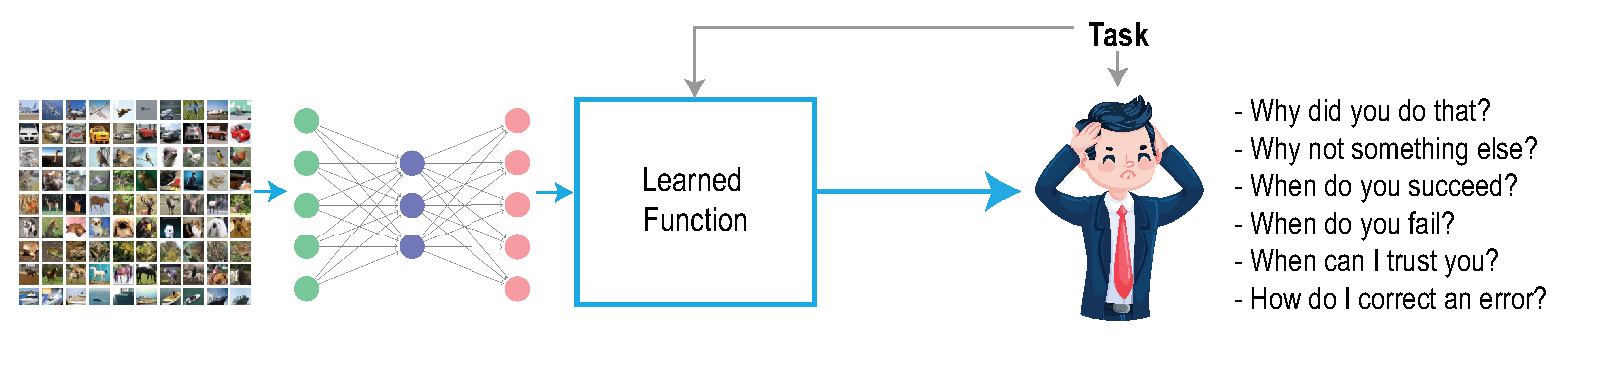
\includegraphics[width=1\textwidth]{images/xa-concept-part-1.eps}
\caption{The Need for Interpretability}
\label{fig:Why Interpretability Matters}
\end{figure}

Without a clear understanding of how and why a model works in a certain way, the development of these models relies on a time consuming trial-and-error process. Consequently, both researchers and practitioners are facing challenges with complex models that demand more transparency and explainable systems to better understanding and analysis of these models. Whether it's an financial decision, a medical decision or maybe a military decision, one cannot rely on a black box method. It's time to act on making these decisions more transparent and understandable before the technology becomes even more pervasive.

The issue of black box neural networks has been a primary concern and a significant focus of discourse in the last few years not only among researchers and practitioners \cite{Samek} but also among businesses operating in regulated industries, such as credit, insurance, legal and benefit systems. 

Over the last few years, algorithmic fairness and accountability has been a matter of concern among consumer advocates, regulators, lawmakers and diversity moderators. An example of this scenario is a 2017 report from the AI Committee of the British Parliament \cite{Hagras2018} that states that the development of the intelligence AI systems is a fundamental necessity if an AI system is to become an integral and trusted tool in the society. Whether it takes the shape of explanation, technological transparency or both depend on the context and stakes involved in its application and sector. However, in most cases, the report makes certain that explainability to be a useful method for the citizens and the consumers. 

Further, the report upholds that it is not acceptable to implement an artificial intelligence system that could have a substantial impact on an individual's life unless it can provide a comprehensive and satisfactory explanation for the decisions it makes. It means delaying their deployment and use for such cases until the system has been vetted and a credible alternative solution is found.

As deep learning spreads across domains, it is of paramount importance that we equip users of deep learning with tools for understanding when a model works correctly, when it fails, and ultimately how to improve its performance. As deep learning more pervasive in public domains, it is essential to be able to verify for a certain task that the accuracy results from the proper framing of a problem statement \cite{Liu2017}, and there is no exploitation of artifacts in the data. Techniques for interpreting and understanding what the model has learned have therefore become a key ingredient of a robust validation procedure \cite{taylor2006methods} \cite{hansen2011visual} \cite{bach2015pixel}. Interpretability is critical in applications such as medical diagnosis, credit approvals and self-driving cars, where the dependency of the model on the correct features should be guaranteed \cite{Caruana:2015:IMH:2783258.2788613} \cite{bojarski2017explaining}.

\subsection{Interpretable Methods}

In this section, I briefly discuss the concept of interpretabiltiy in the context of neural networks and then explore methods for interpreting and understand deep neural networks.

Interpretability is defined as the point to which a human can understand the causes of a decision. Another definition is that interpretability is the degree to which a human can consistently predict the model’s result \cite{molnar}. The higher the interpretability of a machine learning model, the easier it is for someone to understand why certain decisions have been made. A model is better interpretable when its decisions are more accessible for a human to comprehend than decisions made by them \cite{molnar}.

In general, the concept of interpretability center around human understanding and comprehension of object in question. But in the context of neural networks, they vary in the aspect of the model to be understood: its internals, operations, mapping of data, or representation. Although recent work has begun to standardize the definition of interpretability \cite{Lipton2018}, a formal and commonly agreed-upon definition remains open.
    
In our case, interpretability is the process of generating humanly understandable explanations of why a neural network model makes a particular decision \cite{Sacha2017}. Since the learning system hides the entire decision process behind the complicated inner-workings of deep neural networks, it becomes difficult to obtain interpretations and explanations for their decisions.
...Interpretability  is useful in three ways:
[*] UNDERSTANDING
[*] DEBUGGING
[*] REFINEMENT

\subsection{Information Visualization}
[*] RE-STRUCTURE SECTION
[*] More than ever, data visualization has become critical to the field of AI.
Information visualization is the study and usage of visual representation of abstract data to reinforce human cognition. It can help with the discovery of unstructured actionable insight, exploring and understanding the patterns in the data to communicate essential aspects of your data set in a concise, easy-to-understand fashion.

Data analysis is an indispensable part of the machine learning project pipeline, in both business and research projects. The AI development pipeline often begins with data exploration phase, also known as exploratory data analysis to help with data analysis and evaluate approaches for the problem at hand. It has primarily been done using fundamental data analysis approach in visualization such as histograms, plots, charts, graphs and other types.

\subsection{Visualization and Interpretability}

[*] In this section, I highlight key initiatives in the area of machine learning interpretability and review the visualization toolkit and open source libraries available to interpret deep neural networks.

With the growing complexity of AI models and the critical need for understanding their inner-workings has increased. Visualization is potentially a powerful tool to fill this critical need. It can be used to explain the rationales of an AI decisions, including building confidence about how they will behave in the real-world, detecting bias and prejudice, and also for scientific curiosity.

Visualization can played an important role in enhancing the interpretability and explainability of the deep learning models. It provide an in-depth understanding of how deep learning models work. Combined with XAI explanation approach, it can help bring more insight into the often obfuscated complex AI system. It can be used to explain how AI techniques work and help demystify the training and inference process of the model.

Visualizing and interpreting neural network through visualization is currently emerging as a promising research field. it has also attracted research at the intersection of machine learning, information visualization and human-computer interaction (HCI) to build unique solutions with effective human interactions and experience design \cite{Dudley2018}. The growing interest in this field has been reflected in several international conferences and workshops, dedicated exclusively to the topics of interpretability and visualization for machine learning at Visualization for Machine Learning (2018) \cite{visml2018}. These topics has also become the key concerns in panel discussion at premier venues such as NeuRIPS 2016 Workshop on Interpretable ML for Complex Systems \cite{imlcs2016}and ACM Intelligent User Interfaces workshop on Explainable Smart Systems (EXSS 2018) \cite{exss2018}. Besides, there is a growing number of research papers related to visualization and interpretability for deep learning has been published.

[*] CONVNET.JS [*] CITE ANDERJ

[*] CITE BIG PICTURES
TensorFlow Playground is a web-based interactive visualization of neural networks for education and intuitive learning and understanding, where users can play with a basic neural network by changing different configurations such as the width and depth of hidden layers, manage dataset ratio and batch size of dataset, activation type, learning and regularization rate, and types of non-linear activation units. It utilizes two-dimensional toy data sets for problem types such as classification and regression tasks. The manner in which each node in the network is activated across different input data values is fully visualized as a heatmap in a two-dimensional space.

[*] VISDOM
[*] CITE FB
\subsection{Explainable Artificial Intelligence}
Explainable Artificial Intelligence (XAI) is a concept that explains decisions made by the machine learning models and provide justification in a way interpretable by humans \cite{Gunning}. It enables understanding of overall strengths and weaknesses, and conveys an understanding of how the system will behave when implemented in future and how to correct the system’s mistakes \cite{Gunning}.

\begin{figure}[htbp]
\centering
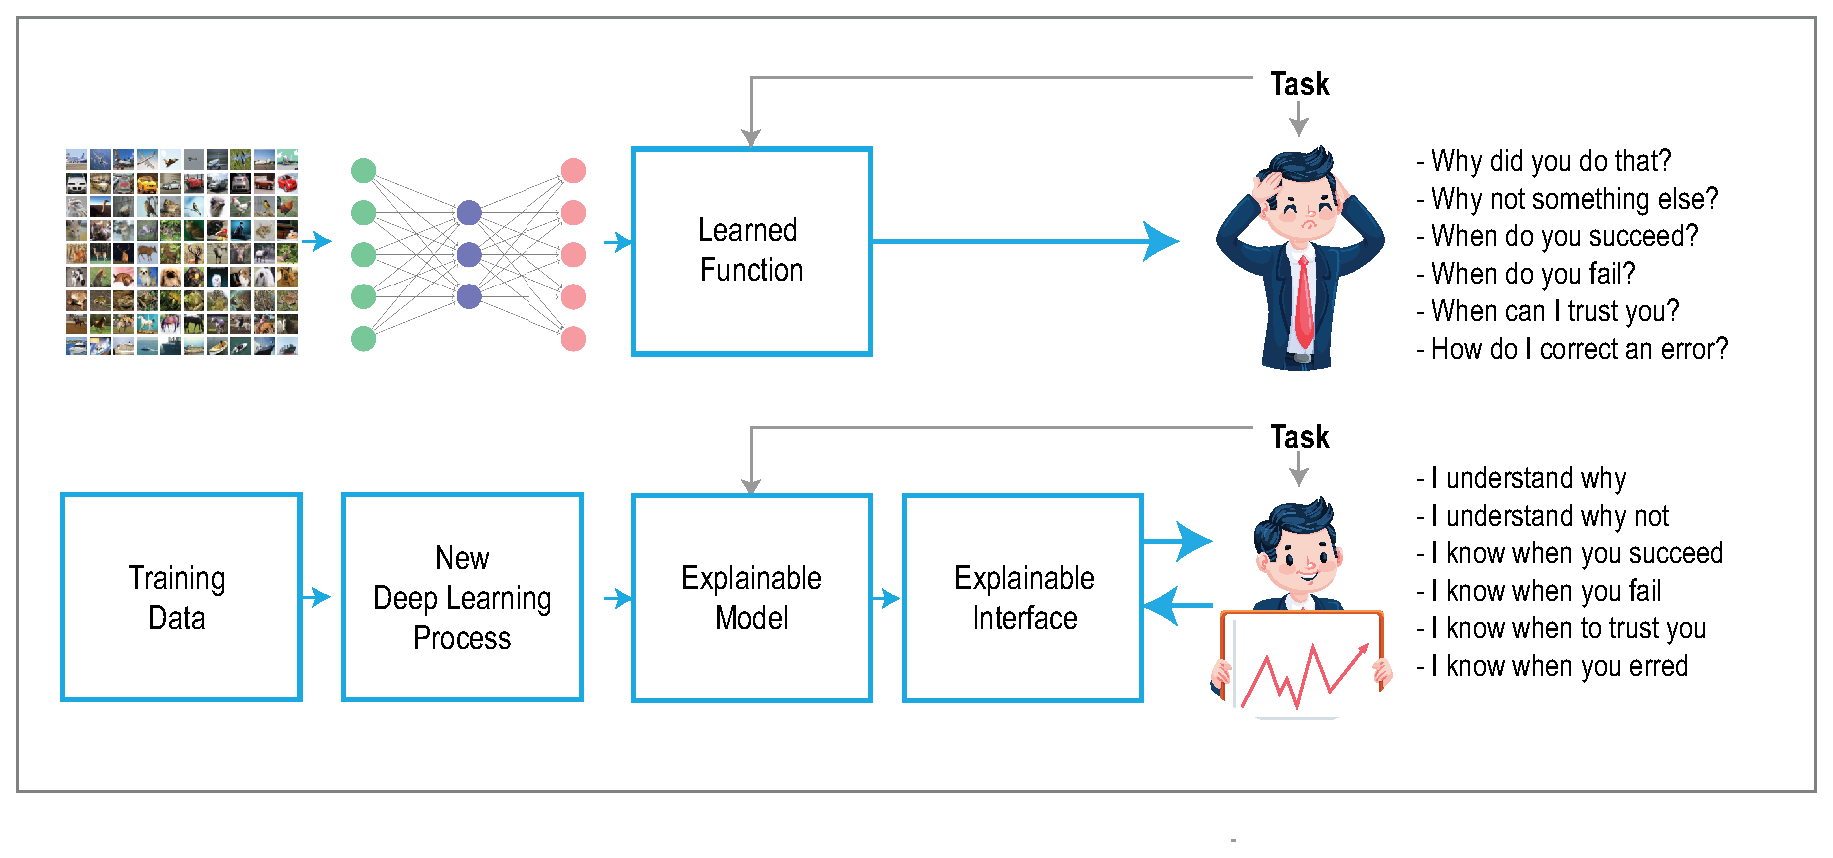
\includegraphics[width=1\textwidth]{images/XAI-concept-copy.eps}
\caption{Explanation framework}
\label{fig:Explanation framework}
\end{figure}

The XAI research and proposals offers a shift towards more transparent and explainable AI system. It aims to create a suite of techniques that produce more interpretable models while maintaining high performance levels. This area of research holds substantial promise for improving trust and transparency of AI-based systems.

The Defense Advanced Research Projects Agency (DARPA), a division of the Defense Department of the United States that explores innovative technologies has launched a large initiative in XAI and funding several projects that aim to make artificial intelligence more interpretable and explainable. The approaches range from adding further machine-learning systems geared toward providing an explanation, to the development of new machine learning techniques where the elucidation is embedded by design. The initiative involves collaboration with research institutes and academic partners to identify challenges in problem areas and develop interpretable models and explainable AI system.

Historically, there has been occasional interest in the explanations of intelligent systems\cite{Abdul}, but the recent successes and proliferation of AI for large-scale applications and the use of increasingly complex and non-transparent algorithms, necessitates another rise of interest for the need to better understand these systems.

The recent wave of interest in explainable artificial intelligence can be attributed to the latest efforts by the DARPA's initiative to fund XAI projects. As defense intelligent agents and military operations may come to rely heavily on machine learning to parse huge quantities of data from satellite imagery, radio signals and other sensors, and to control a growing equipment of autonomous systems. US military wants to take pre-emptive measure to ensure that this reliance doesn’t lead to blindly trusting in any type of algorithms. It might not matter that much if the new machine learning technique is opaque but not in the case of a military commander trying to identify a potential target \cite{Knight2017} or an intelligence officer surveilling cyberespionage by a foreign agent.

DARPA program managers recognizes that there is a real advancement happening in AI and that these models are very opaque and difficult for people to interpret, especially if they are not an expert in AI \cite{Knight2017}. Thereupon, they are committed to helping develop AI techniques that provide explanation for their reasoning.

DARPA is funding several research groups, which are pursuing a range of approach and techniques to make AI models more explainable. Recently, it released Explainable Artificial Intelligence (DAR, 2016) to encourage research on this topic \cite{Gunning}. The main goal of XAI is to create a suite of machine learning techniques that produce explainable models to enable users to understand, trust, and manage the emerging generation of Artificial Intelligence systems \cite{Gunning2}.

Furthermore, military will be developing several autonomous systems in the coming years that will undoubtedly rely heavily on machine learning techniques like deep learning. Self driving military vehicles, along with aerial drones will be deployed and they will become increasingly capable over time.

\begin{figure}[htbp]
\centering
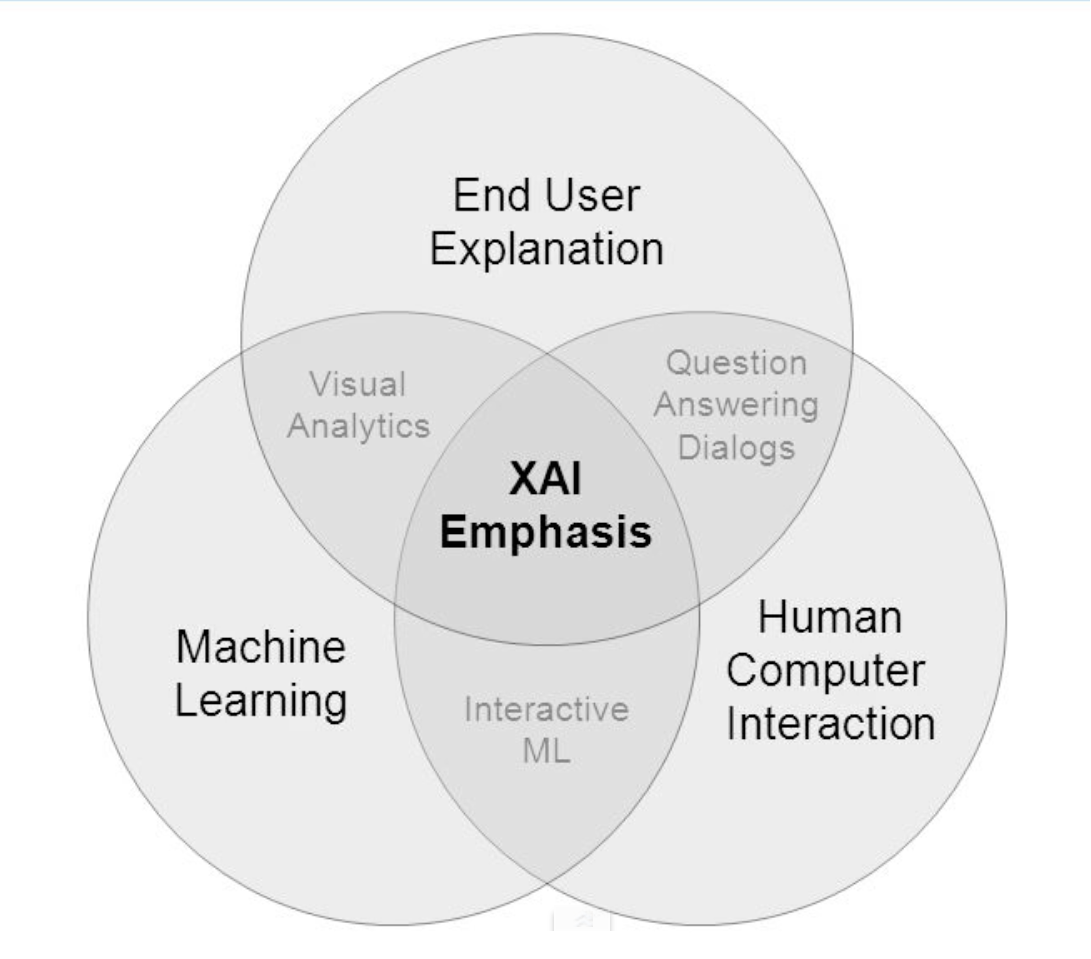
\includegraphics[width=0.5\textwidth]{images/XAI-research-1-crop.png}
\caption{Emphasis and Scope of XAI Research}
\label{fig:xai-1}
\end{figure}

XAI has been gaining increasing attention lately with several conference series dedicated exclusively to the topic of interpretability, transparency, fairness and accountability. Broadly, XAI landscape can be divided into two research groups (i) a group of academic institutions, non-profit research labs and firms in the regulated industries (such as credit, insurance and legal system) and (ii) civilian and military researchers funded by DARPA. The former group is mainly focused on promoting fairness and transparency in algorithmic decision-making with social and commercial impact.

\section{Deep Learning Visualization Research}

%With the growing complexity of AI models, the critical need for understanding their inner-workings has increased. Visualization is potentially a powerful technique to fill such a critical need. It can help bring more insight into the often obfuscated complex AI systems.

Deep learning visualization research is an interdisciplinary area spanning multiple related fields within and outside deep learning and AI community \cite{Choo2018}. In academia, the the primary venue for deep learning visualization research consists of two main groups (1) Information Visualization and Visual Analytics community; and (2) artificial intelligence and deep learning communities. These two groups occasionally also coordinate with human-computer interaction communities, which in turn is a multi-disciplinary field of computer science, cognitive science, human-factor engineering, design and others.

In this section, I discuss the research questions that formed the basis of of research process, and discuss them using the human-centered framework, which is organized around various facets of the deep learning visualization research.



It can potentially help three broad groups of practitioners and users of AI who stand to benefit from deep learning visualization and visual analytics: model developers, model users, and non-experts \cite{Choo2018}.

Deep learning visualization research is an interdisciplinary area involving both deep learning and visual analytics techniques \cite{Choo2018}. It is distributed across multiple related fields within and outside the deep learning and AI community. In academia, the primary venue for deep learning visualization research consists of two main groups (1) Information Visualization and Visual Analytics community; and (2) artificial intelligence and deep learning communities. 

In addition to that, since this area is relatively new and emerging \cite{Choo2018}, it has seen more attention at multiple conferences and workshops, such as Neural Information Processing Systems (NeurIPS), IEEE Transactions on Visualization, IEEE Information Visualization and Computer Graphics and ICML Workshop on Human Interpretability in ML as just to name a few examples.

\subsection{Visual Analytics System}
    
Visual Analytics combines information visualization and scientific visualization and focuses on the analytical reasoning enabled with interactive visual interfaces. It’s an amalgamation of computer science, information visualization, cognitive and perceptual sciences, interactive design and social science.

Visual Analytics systems have been developed to inspect artificial neural networks since visual feedback is considered highly valuable by both the practitioners and researchers.

================================================
Although recent visual analytics systems provide sophisticated visualization and interaction capabilities, research issues on how to effectively loop human into the analysis process and how to increase applicability of explainable deep learning techniques have not been fully investigated. For example, widening user interaction capabilities with deep learning models based on various user needs, tightly integrating the current data-driven learning process with knowledge-driven analysis processes, evaluating and improving the robustness of deep learning against out-of- sample data, as well as explaining other types of popular deep learning models, still pose considerable challenges for explainable deep learning

